%% History:
% Pavel Tvrdik (26.12.2004)
%  + initial version for PhD Report
%
% Daniel Sykora (27.01.2005)
%
% Michal Valenta (3.12.2008)
% rada zmen ve formatovani (diky M. Duškovi, J. Holubovi a J. Žďárkovi)
% sjednoceni zdrojoveho kodu pro anglickou, ceskou, bakalarskou a diplomovou praci

\documentclass[12pt,twoside,a4paper]{book}   %two-page printing
\usepackage[czech, english]{babel}
\usepackage[T1]{fontenc} % pouzije EC fonty
\usepackage[utf8]{inputenc}
\usepackage{graphicx}
%\usepackage{indentfirst} %1. odstavec jako v cestine.


\usepackage{k336_thesis_macros} % specialni makra pro formatovani DP a BP
 % muzete si vytvorit i sva vlastni v souboru k336_thesis_macros.sty
 % najdete  radu jednoduchych definic, ktere zde ani nejsou pouzity
 % napriklad: 
 % \newcommand{\bfig}{\begin{figure}\begin{center}}
 % \newcommand{\efig}{\end{center}\end{figure}}
 % umoznuje pouzit prikaz \bfig namisto \begin{figure}\begin{center} atd.


%%%%%%%%%%%%%%%%%%%%%%%%%%%%%%%%%%%%%
% Zvolte jednu z moznosti 
% Choose one of the following options
%%%%%%%%%%%%%%%%%%%%%%%%%%%%%%%%%%%%%
\newcommand\TypeOfWork{Diplomová práca} \typeout{Diplomova prace}
% \newcommand\TypeOfWork{Master's Thesis}   \typeout{Master's Thesis} 
% \newcommand\TypeOfWork{Bakalářská práce}  \typeout{Bakalarska prace}
% \newcommand\TypeOfWork{Bachelor's Project}  \typeout{Bachelor's Project}


%%%%%%%%%%%%%%%%%%%%%%%%%%%%%%%%%%%%%
% Zvolte jednu z moznosti 
% Choose one of the following options
%%%%%%%%%%%%%%%%%%%%%%%%%%%%%%%%%%%%%
% nabidky jsou z: http://www.fel.cvut.cz/cz/education/bk/prehled.html

%\newcommand\StudProgram{Elektrotechnika a informatika, dobíhající, Bakalářský}
%\newcommand\StudProgram{Elektrotechnika a informatika, dobíhající, Magisterský}
% \newcommand\StudProgram{Elektrotechnika a informatika, strukturovaný, Bakalářský}
 \newcommand\StudProgram{Elektrotechnika a informatika, strukturovaný, Navazující magisterský}
% \newcommand\StudProgram{Softwarové technologie a management, Bakalářský}
% English study:
% \newcommand\StudProgram{Electrical Engineering and Information Technology}  % bachelor programe
% \newcommand\StudProgram{Electrical Engineering and Information Technology}  %master program


%%%%%%%%%%%%%%%%%%%%%%%%%%%%%%%%%%%%%
% Zvolte jednu z moznosti 
% Choose one of the following options
%%%%%%%%%%%%%%%%%%%%%%%%%%%%%%%%%%%%%
% nabidky jsou z: http://www.fel.cvut.cz/cz/education/bk/prehled.html

%\newcommand\StudBranch{Výpočetní technika}   % pro program EaI bak. (dobihajici i strukt.)
\newcommand\StudBranch{Výpočetní technika}   % pro prgoram EaI mag. (dobihajici i strukt.)
%\newcommand\StudBranch{Softwarové inženýrství}            %pro STM
%\newcommand\StudBranch{Web a multimedia}                  % pro STM
%\newcommand\StudBranch{Computer Engineering}              % bachelor programe
%\newcommand\StudBranch{Computer Science and Engineering}  % master programe


%%%%%%%%%%%%%%%%%%%%%%%%%%%%%%%%%%%%%%%%%%%%
% Vyplnte nazev prace, autora a vedouciho
% Set up Work Title, Author and Supervisor
%%%%%%%%%%%%%%%%%%%%%%%%%%%%%%%%%%%%%%%%%%%%

\newcommand\WorkTitle{Model siete ZigBee}
\newcommand\FirstandFamilyName{Bc. Bernard Halás}
\newcommand\Supervisor{doc. Ing. Jan Janeček, CSc}


% Pouzijete-li pdflatex, tak je prijemne, kdyz bude mit vase prace
% funkcni odkazy i v pdf formatu
\usepackage[
pdftitle={\WorkTitle},
pdfauthor={\FirstandFamilyName},
bookmarks=true,
colorlinks=true,
breaklinks=true,
urlcolor=red,
citecolor=blue,
linkcolor=blue,
unicode=true,
]
{hyperref}




\begin{document}

%%%%%%%%%%%%%%%%%%%%%%%%%%%%%%%%%%%%%
% Zvolte jednu z moznosti 
% Choose one of the following options
%%%%%%%%%%%%%%%%%%%%%%%%%%%%%%%%%%%%%
\selectlanguage{czech}
%\selectlanguage{english} 

% prikaz \typeout vypise vyse uvedena nastaveni v prikazovem okne
% pro pohodlne ladeni prace


\iflanguage{czech}{
	 \typeout{************************************************}
	 \typeout{Zvoleny jazyk: cestina}
	 \typeout{Typ prace: \TypeOfWork}
	 \typeout{Studijni program: \StudProgram}
	 \typeout{Obor: \StudBranch}
	 \typeout{Jmeno: \FirstandFamilyName}
	 \typeout{Nazev prace: \WorkTitle}
	 \typeout{Vedouci prace: \Supervisor}
	 \typeout{***************************************************}
	 \newcommand\Department{Katedra počítačů}
	 \newcommand\Faculty{Fakulta elektrotechnická}
	 \newcommand\University{České vysoké učení technické v Praze}
	 \newcommand\labelSupervisor{Vedúci práce}
	 \newcommand\labelStudProgram{Študíjny program}
	 \newcommand\labelStudBranch{Obor}
}{
	 \typeout{************************************************}
	 \typeout{Language: english}
	 \typeout{Type of Work: \TypeOfWork}
	 \typeout{Study Program: \StudProgram}
	 \typeout{Study Branch: \StudBranch}
	 \typeout{Author: \FirstandFamilyName}
	 \typeout{Title: \WorkTitle}
	 \typeout{Supervisor: \Supervisor}
	 \typeout{***************************************************}
	 \newcommand\Department{Department of Computer Science and Engineering}
	 \newcommand\Faculty{Faculty of Electrical Engineering}
	 \newcommand\University{Czech Technical University in Prague}
	 \newcommand\labelSupervisor{Supervisor}
	 \newcommand\labelStudProgram{Study Programme} 
	 \newcommand\labelStudBranch{Field of Study}
}




%%%%%%%%%%%%%%%%%%%%%%%%%%    Poznamky ke kompletaci prace
% Nasledujici pasaz uzavrenou v {} ve sve praci samozrejme 
% zakomentujte nebo odstrante. 
% Ve vysledne svazane praci bude nahrazena skutecnym 
% oficialnim zadanim vasi prace.

%%%%%%%%%%%%%%%%%%%%%%%%%%    Titulni stranka / Title page 

\coverpagestarts

%%%%%%%%%%%%%%%%%%%%%%%%%%%    Podekovani / Acknowledgements 

\acknowledgements
\noindent
Rád by som sa poďakoval pánu Janečkovi za konzultácie, pripomienky a návrhy, ktoré mi ochotne poskytol počas vypracovávania tejto práce. Takisto vďaka patrí aj mojej rodine za podporu počas celého obdobia môjho štúdia.


%%%%%%%%%%%%%%%%%%%%%%%%%%%   Prohlaseni / Declaration 

\declaration{V Prahe dňa 21.\,5.\,2009}
%\declaration{In Kořenovice nad Bečvárkou on May 15, 2008}


%%%%%%%%%%%%%%%%%%%%%%%%%%%%    Abstract 
 
\abstractpage

Translation of Czech abstract into English.

% Prace v cestine musi krome abstraktu v anglictine obsahovat i
% abstrakt v cestine.
\vglue60mm

\noindent{\Huge \textbf{Abstrakt}}
\vspace{8ex}

\noindent
Abstrakt práce by měl velmi stručně vystihovat její podstatu. Tedy čím se práce zabývá a co je jejím výsledkem/přínosem.

\noindent
Očekávají se cca 1 -- 2 odstavce, maximálně půl stránky.

%%%%%%%%%%%%%%%%%%%%%%%%%%%%%%%%  Obsah / Table of Contents 

\tableofcontents


%%%%%%%%%%%%%%%%%%%%%%%%%%%%%%%  Seznam obrazku / List of Figures 

\listoffigures


%%%%%%%%%%%%%%%%%%%%%%%%%%%%%%%  Seznam tabulek / List of Tables

\listoftables


%**************************************************************

\mainbodystarts
% horizontalní mezera mezi dvema odstavci
%\parskip=5pt
%JZ 11.12.2008 parskip bez tolerance? To neni rozumne, myslel jsem, ze sazime v TeXu, ne ve Wordu!
\parskip=5pt plus 4pt minus 4pt
% odstazeni prvniho radku odstavce (neaplikuje se na prvni odstace 
% kapitol, sekci, podsekci atd.)
%\parindent=10pt
%JZ 11.12.2008 -- indent v zavislosti na base font, proc 10pt?
\parindent=1.5em
% pokud chcete selektivne zamezit odsazeni 1. radku nektereho odstavce
% pouzijte prikaz \noindent.

%**************************************************************

% Pro snadnejsi praci s vetsimi texty je rozumne tyto rozdelit
% do samostatnych souboru nejlepe dle kapitol a tyto potom vkladat
% pomoci prikazu \include{jmeno_souboru.tex} nebo \include{jmeno_souboru}.
% Napr.:
% \include{1_uvod}
% \include{2_teorie}
% atd...

%*****************************************************************************
\cleardoublepage\chapter{Úvod}

\indent\indent Od napísania mojej prvej práce zaoberajúcej sa simuláciami senzorových sietí~\cite{halas03} uplynuli približne tri roky. Technológia sa posunula o malý krok vpred a zariadenia pre komunikáciu v senzorových sieťach nenáročných na šírku datového prenosu sa stávajú cenovo dostupnejšie. Vynárajú sa otázky, či pri masívnejších nasadeniach sú tieto siete schopné vykonávať požadované úlohy pri zdieľaní prenosového média spolu s takisto čoraz rozšírenejšími technológiami bezdrôtových sietí ako Wi-Fi$^{TM}$, alebo Bluetooth$^{TM}$, s ktorými zdieľajú časti frekvenčného spektra pre svoju komunikáciu.\\
\indent Na základe týchto skutočností sa ponúkalo zúročiť získané skúsenosti so simulačnými systémami a pripraviť aktuálnejší model siete ZigBee postavenej nad technológiou IEEE 802.15.4$^{TM}$, ktorý by reflektoval zmeny štandardov z uplynulých mesiacov a rokov a ktorý by ponúkal bohatšie možnosti simulácii s výsledkami bližšími reálnemu svetu.

\cleardoublepage\chapter{Špecifikácia požiadaviek na navrhovaný systém}

\section{Popis problému}
\indent\indent Špecifikácia siete ZigBee~\cite{zigbee08} predstavuje uzavretý dokument popisujúci udalosti, procesy a obsah komunikácie medzi jednotlivými modulmi v rámci hierarchie definovanej takisto týmto dokumentom. Štandard ZigBee hovorí o vyšších sieťových vrstvách. Vynecháva fyzickú a linkovú vrstvu. V daných prípadoch sa spolieha na iný dokument, na špecifikáciu protokolu IEEE 802.15.4\texttrademark~\cite{ieee06}.\\
\indent\indent Informácie obsiahnuté v týchto dvoch dokumentoch je nutné premietnuť do vnú\-tornej štruktúry modelov simulátora pre získanie čo najvernejších výsledkov. Od modelu sa takisto očakáva reflektovanie nárokov vkladaných do reálnych sietí, a to mobilita daných prvkov, ktorá nie je bezdrôtovým senzorových sietí cudzia a určite zakomponovanie javov sprevádzajúcich šírenie elektromagnetického signálu vzduchom. Z experimentálnej stránky veci nás zaujíma aj možnosť nasadenia technológie TCP/IP nad technológiami ZigBee/IEEE 802.15.4

\section{Požiadavky na model}
\indent\indent Požiadavky kladené na simulačný model by sa dali zhrnúť do nasledujúcich niekoľko bodov:
\begin{enumerate}
  \item Obsiahnutie základných vlastností deklarovaných v štandardoch ZigBee a IEEE 802.15.4
  \item Podpora mobility všetkých sieťových prvkov
  \item Zahrnutie vplyvov prostredia (interferencia, šum, ...)
  \item Pripraviť rozhranie umožňujúce prenos IP (Internet Protocol) paketov
  \item Modularita pre ľahké aktualizácie modelu v prípade vydania nových verzii štandardov
  \item Výpočtová náročnosť vykonávaných simulácii v rozumných medziach
\end{enumerate}
\subsection{Vlastnosti sietí postavených na IEEE 802.15.4}
\indent\indent Štandard uvedený technickej verejnosti v roku 2003 špecifikuje fyzickú a linkovú vrstvu Low-Rate WPAN (Wireless Personal Area Network) sietí. Charakteristické vlastnosti týchto sietí sú nízka spotreba, nízka dátová priepustnosť, v prípade potreby garancia istého prenosového pásma a jednoduchosť jednotlivých procesov, z ktorej vyplývajú nevysoké požiadavky na riadiace procesory. Typická aktivita v čase zariadení tohoto typu je pod 0.1\%. Elementy, ktoré sú pri takto nastavených požiadavkách na sieť potrebné pre jej efektívne fungovanie a bez ktorých sa náš simulačný model nezaobíde sú nasledovné:
\begin{description}
  \item[RFD/FFD prvky] (Full Functionality Device, Reduced Functionality Device) prvky siete IEEE sa podľa funkčnosti delia na dve hlavné skupiny. Konštrukčne jednoduchšie označujeme ako RFD. V teórii grafov by sme ich vďaka ich polohe v stromovej topológii označili listami. Odpoveď na to, prečo potrebujeme zložité (FFD) a jednoduché prvky (RFD) je v tom, že v rámci stromovej hierarchie len tie zariadenia nachádzajúce sa vyššie majú svoju úlohu doplnenú o posielanie beacon rámcov, smerovanie paketov, prijímanie žiadostí o asociáciu siete a pod.
  \item[Beacon rámce] sú rámce vysielané v pravidelných intervaloch zariadením typu FFD a majú za úlohu informovať o plánovaných dátových prenosoch, topológii a~o~konfiguračných premenných danej siete. Tieto rámce sa objavujú pravidelne a vďaka tomu príjemca vie, kedy si môže dovoliť vypnúť prijímač mikrovlnného signálu s cieľom šetriť energiu s istotou nepremeškania žiadneho beacon rámca.
  \item[CSMA-CA] (Carrier Sense Multiple Access - Collision Avoidance) je metóda prístupu k zdieľanému médiu. V našom prípade je médiom vzduch a metóda nám pomáha vyvarovať sa kolízii rámcov pri ich vysielaní a príjme.
  \item[GTS mechanizmus] (Guaranteed Time Slot) je systém periodického rezervovania časových slotov pre posielanie rámcov medzi prvkami v stromovej topológii. Môže byť v prípade potreby zárukou získania určitej šírky prenosového pásma pre jednotlivé sieťové prvky, a~teda umožňovať komunikáciu s nízkou latenciou.
 \end{description}
\indent\indent O týchto vlastnostiach a o spôsobe ich prípadnej implementácie si povieme viac v neskorších kapitolách.
\subsubsection{Mobilita}
\indent\indent Na sieťové prvky bezdrôtových sietí je často kladený požiadavok mobility daného prvku v priestore, ktorý je v konečnom dôsledku premietaný do úprav pozície daného prvku v topológii siete. Pre simulátor teda vyplýva, že musí dynamicky v čase vedieť polohu prvku pre výpočet hodnôt fyzikálnych veličín charakterizujúcich prenos a následný príjem signálu.\\
\indent Čo sa týka daného modelu, ten by mal mať schopnosť reagovať v prípade, že komunikačné cesty po zmene polohy už nie sú schopné dostatočne kvalitne prenášať rámce. Toto je vlastnosť prvkov, na ktorú sa v špecifikácii~\cite{ieee06} myslí, a teda vo finálnom modeli bude zahrnutá.
\subsubsection{Vlastnosti prenosového média}
\indent\indent Siete, ktoré sú predmetom nášho záujmu, pristupujú k zdieľanému médiu - vzduchu. Tým, že médium je spoločné pre všetky prvky siete, stav, v ktorom sa nachádza, má rôznou mierou vplyv na všetky prijímače elektromagnetického signálu. Mnohé simulátory sa zameriavajú práve na verné spracovanie tejto skutočnosti. Ich metódy napríklad pre výpočet prijímaného výkonu, alebo odstupu signálu od šumu (SNR) sú výborne spracované a budú pre náš simulátor užitočné.
\subsection{Modularita návrhu}
\indent\indent Podobne ako v predchádzajúcej práci~\cite{halas03} sa nám overil diferencovaný prístup k jednotlivým vrstvám  odvodený od OSI-ISO modelu, tiež teraz budú jednotlivé sieťové prvky zložené z viacerých modulov, ktoré budú medzi sebou komunikovať ideálne len predávaním správ.\\
\indent Tento pohľad na komplexnú štruktúru sieťových prvkov nám zaručí jednoduchosť prípadných neskorších zásahov napríklad z dôvodu úprav v smerovacích mechanizmoch. V danom prípade bude nutné iba vykonať zmeny v module, ktorý zabezpečuje smerovanie paketov.


\cleardoublepage\chapter{Zigbee a IEEE 802.15.4}

\indent\indent S nástupom zariadení pre bezdrôtovú komunikáciu určených pre použitie v lokálnych (LAN - Local Area Network), alebo osobných (PAN - Personal Area Network) sieťach sa začala vynárať možnosť využiť bezdrôtovú technológiu aj pre inteligentné systémy, ktoré nevyžadujú vysoké prenosové rýchlosti. To bol popud pre vznik štandardu pre bezdrôtovú komunikáciu v LAN a PAN sieťach charakteristickú nízkymi prenosovými rýchlosťami, malými nárokmi na konfiguráciu a aj samotnú prevádzku.\\

\section{IEEE 802.15.4}
\indent\indent Tento štandard definujúci fyzickú (PHY - Physical) a linkovú (MAC - Media Access Control) vrstvu bol prvý krát predstavený v roku 2003~\cite{ieee03}. Od toho momentu je ďalej vyvíjaný dvoma smermi. Jeden bol predstavený v roku 2006 pod označením IEEE 802.15.4b~\cite{ieee06}, formálne aj označovaný ako IEEE 802.15.4b-2006 vďaka roku svojho publikovania. Rozšíril možnosti modulácie signálu, a teda aj zvýšil maximálne prenosové rýchlosti vo frekvenčných pásmach 868/915~MHz. Umožnenie viacerých druhov modulácie v týchto prenosových pásmach umožnilo zjednodušenie samotných zariadení, pretože na komunikáciu v 868/915~MHz a 2.4 GHz už stačil iba jeden modulačný čip. Druhú vetvu vývoja prestavoval štandard označovaný ako IEEE 802.15.4a prípadne formálne IEEE 802.15.4a-2007, ktorý operuje v pásme Ultra-Wideband (UWB). Týmto sa však nebudeme v tejto práci zaoberať. Všetky nasledovné informácie sa budú viazať k verzii IEEE 802.15.4b-2006, ak nebude uvedené inak.\\
\indent Siete postavené podľa IEEE 802.15.4b-2006 sú charakteristické tým, že ponúkajú
\begin{itemize}
\item Prevádzku v bezlicencovaných frekvenčných pásmach
\item Prenosové rýchlosti na úrovniach 250, 100, 40, alebo 20 kb/s
\item Topológiu v tvare hviezda (star), alebo každý s každým (peer-to-peer)
\item Komunikáciu pomocou 64-bitových, alebo 16-bitových adries
\item Mechanizmus alokácie časových slotov (GTS)
\item Prístup na médium vyhýbajúci sa kolíziám (CSMA-CA)
\item Spoľahlivý prenos dát s mechanizmom kotroly integrity (FCS - Frame Check Sequence) a potvrdzovaním dát
\item Aktivitu zariadení priemerne na úrovni 0.1\% doby cyklu
\end{itemize}
\indent Všeobecne, IEEE 802.15.4 predstavuje základ pre tzv. LR-WPAN (Low-Rate Wireless PAN) siete. Naň sa spoliehajú technológie ako WirelessHART, MiWi, alebo aj ZigBee.\\
\subsection{Topológia}
\indent\indent Pre vytvorenie PAN siete je potrebné, aby minimálne jeden z prvkov bol typu FFD. Tieto zariadenia majú schopnosť vytvárať WPAN sieť (v prípade, že fungujú aj ako PAN koordinátor), okrem toho aj prideľujú sieťové adresy, asociujú nové prvky do siete a vysielajú tzv. beacon rámce.\\
\indent Prvky FFD a RFD môžu tvoriť 2 druhy usporiadaní z pohľadu topológie siete - hviezdu a každý s každým.\\
\subsubsection{Hviezda (Star)}
\indent\indent Siete typu Hviezda fungujú na sebe nezávisle a bez problémov ich môže operovať viac vo svojom vzájomnom dosahu. Každá z nich musí byť ale jednoznačne identifikovateľná svojím PAN identifikátorom. V centre siete je PAN koordinátor. Zariadenie, či už FFD, alebo RFD si pri pripájaní do siete môže vybrať ľubovoľný PAN koordinátor vo svojom dosahu a požiadať ho o asociáciu. Príklad takejto siete je zobrazený na obrázku~\ref{fig:topology_star}.\\
\begin{figure}[htbp]
\begin{center}
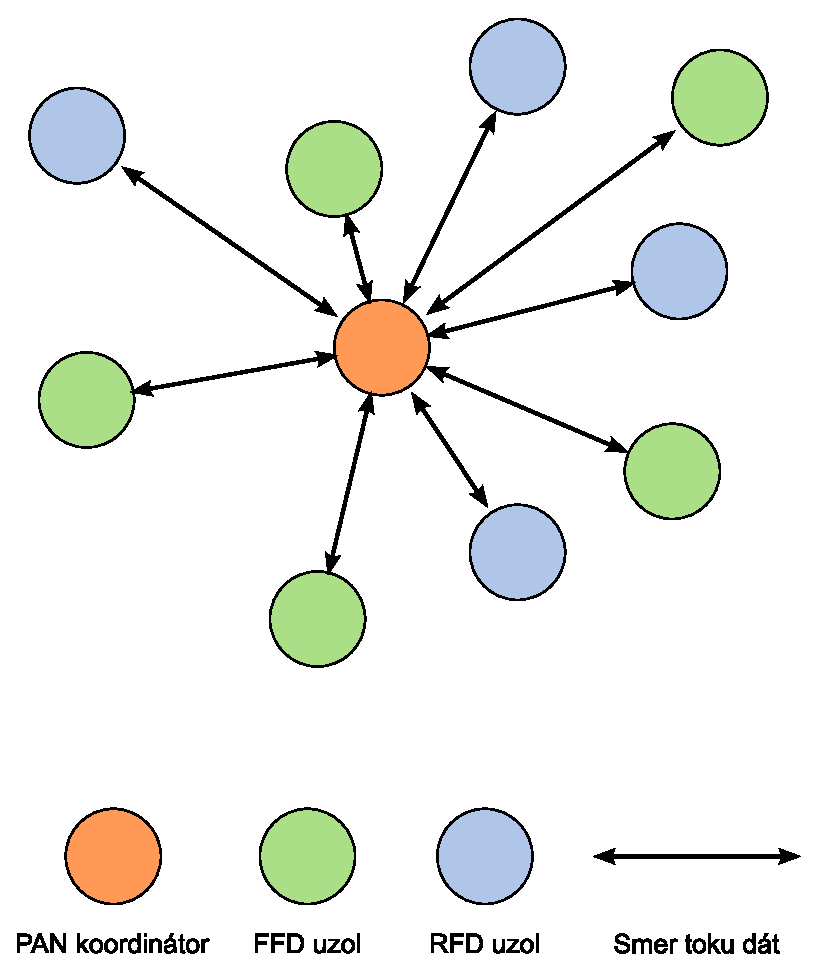
\includegraphics[width=120mm]{figures/topology_star}
\caption{Topológia typu hviezda}
\label{fig:topology_star}
\end{center}
\end{figure} 
\subsubsection{Každý s každým (Peer-to-Peer)}
\indent\indent V tomto type topológie je implementovaná ide aby mohlo každé zariadenie komunikovať s ľubovoľným iným vo svojom dosahu. Takisto v takýchto sieťach existuje jeden FFD prvok v roli PAN koordinátora. Ukážka na obrázku~\ref{fig:topology_p2p}.\\
\begin{figure}[htbp]
\begin{center}
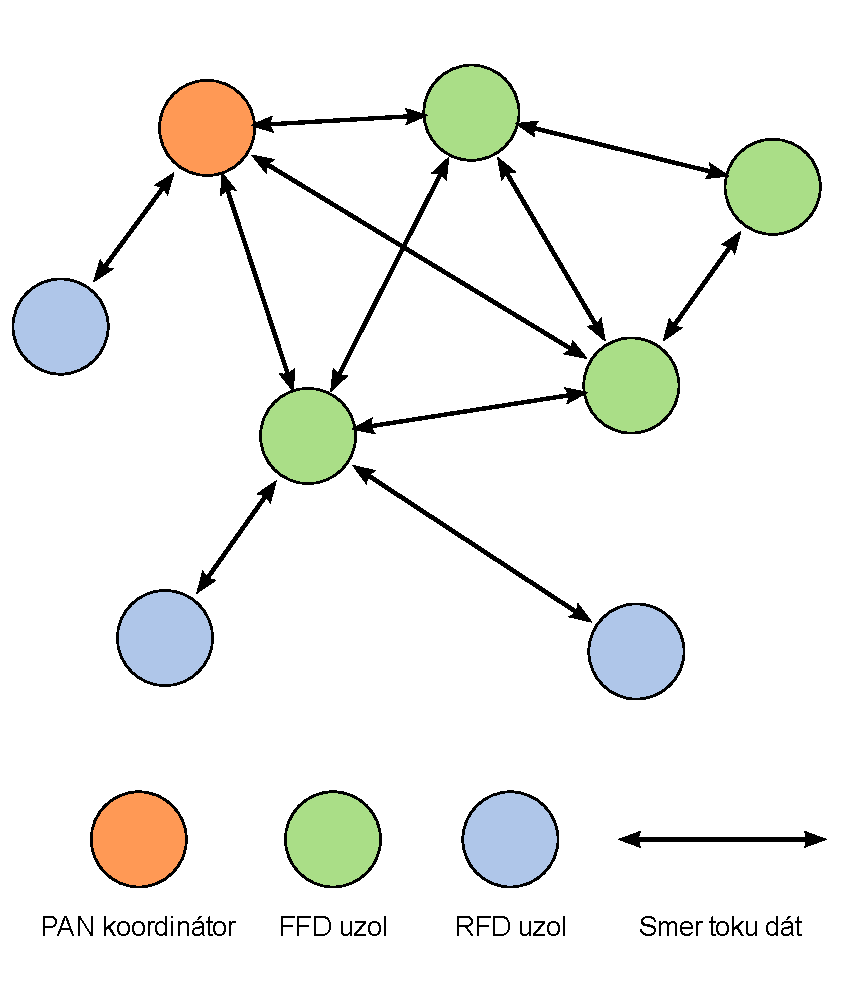
\includegraphics[width=120mm]{figures/topology_p2p}
\caption{Topológia typu každý s každým}
\label{fig:topology_p2p}
\end{center}
\end{figure} 
\indent Z tohoto typu sietí je odvodený variant Zhluk stromov (Cluster Tree). V takejto topológii je prevažná väčšina zariadení typu FFD. Zariadenia typu RFD sa pripájajú k~stromu ako listy. Všetky FFD sú schopné vysielať synchronizačné beacon rámce. Z~nich môže byť však len jeden PAN koordinátor. Ak bude asociácia zariadenia do siete z~nejakého dôvodu odmietnutá, prvok môže vyhľadať iné FFD zariadenie a skúsiť asociáciu u~neho.\\
\indent V prípade, že sú splnené určité podmienky, PAN koordinátor môže požiadať FFD prvok v rámci svojej siete, aby  zformoval novú PAN sieť s novým identifikátorom. Ostatné zariadenia sa potom môžu pripájať až budú tvoriť podobné štruktúry, ako je tá na obr.~\ref{fig:topology_cluster}. Volá sa zhluk stromov (Cluster Tree) Takáto konfigurácia ponúka plošne široké pokrytie, na druhú stranu však správy pri prechode cez viaceré PAN zvyšujú svoju latenciu.\\
\begin{figure}[htbp]
\begin{center}
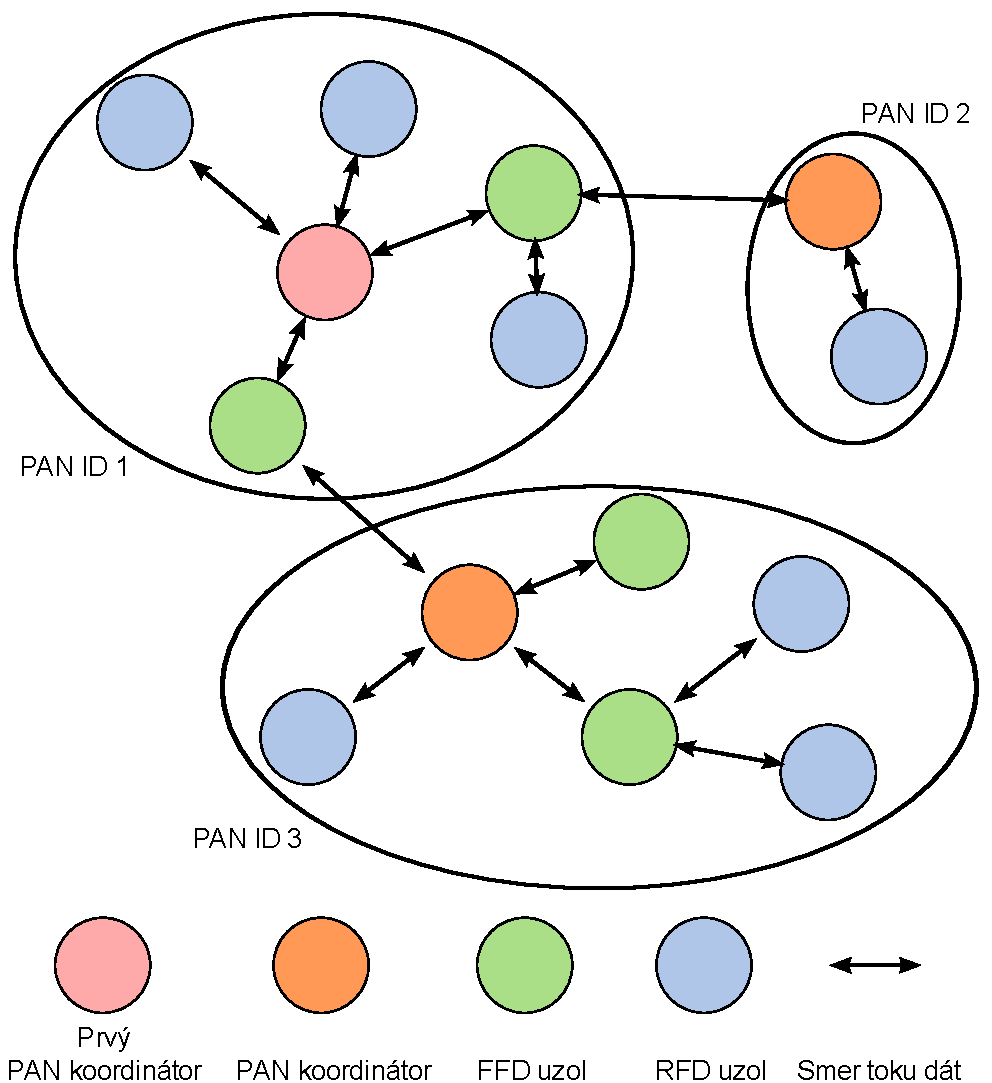
\includegraphics[width=120mm]{figures/topology_cluster}
\caption{Topológia typu zhluk stromov}
\label{fig:topology_cluster}
\end{center}
\end{figure} 
\subsection{Fyzická vrstva}
\indent\indent Ako už bolo spomenuté, jedná sa o technológiu pracujúcu so vzduchom ako zdieľaným médiom. Frekvenčné pásma, v ktorých zariadenia operujú, sú uvedené v tabuľke~\ref{tab:frequencies}. Je vhodné podotknúť, že sa jedná o tzv. bezlicencované (ISM - Industrial Scientific and Medical) pásma, avšak kým 2.4 GHz je s malými obmedzeniami k dispozícii takmer po celom svete, pásmo ISM 868~MHz je len v Európe a ISM 902-928~MHz je k dispozícii len v USA.\\
\begin{table}[htbp]
\begin{center}
\begin{tabular}{|c|c|l|c|c|l|}
  \hline
  \multirow{2}{*}{\textbf{PHY}} & \multirow{2}{*}{\textbf{Frekvencia}} & \multirow{3}{*}{\textbf{Modulácia}} & \textbf{Prenosová} & \textbf{Symbol} & \multirow{3}{*}{\textbf{Symboly}} \\ 
  \multirow{2}{*}{(MHz)} & \multirow{2}{*}{(MHz)} & & \textbf{rýchlosť} & \textbf{rate} & \\ 
  & & & (kbps) & (ksym/s) & \\ [0.5ex]
  \hline\hline
  \multirow{2}{*}{868/915} & 868--868.6 & BPSK & 20 & 40 & Binárne\\
  & 902--928 & BPSK & 40 & 40 & Binárne\\ [0.5ex]
  \hline
  \multirow{2}{*}{868/915} & 868--868.6 & ASK & 250 & 12.5 & 20-bitové PSSS\\
  & 902--928 & ASK & 250 & 50 & 5-bitové PSSS\\ [0.5ex]
  \hline
  \multirow{2}{*}{868/915} & 868--868.6 & O-QPSK & 100 & 25 & 16-kové ortogonálne\\
  & 902--928 & O-QPSK & 250 & 62.5 & 16-kové ortogonálne\\ [0.5ex]
  \hline
  2450 & 2400--2483.5 & O-QPSK & 250 & 62.5 & 16-kové ortogonálne\\ [0.5ex]
  \hline
\end{tabular}
\caption{Používané frekvenčné pásma, modulácie a kódové symboly}
\label{tab:frequencies}
\end{center}
\end{table}
\indent\indent Pre komunikáciu je vyhradených 27 kanálov, ktoré sú združené do troch tzv. stránok kanálov. Takýto spôsob členenia je z historických dôvodov a z dôvodov spätnej kompatibility so zariadeniami fungujúcimi na IEEE 802.15.4-2003. Stránky sú očíslované v rozsahu 0--31, pričom v aktuálne sú stránky 3--31 rezervované do budúcna.\\ 
\indent Na definovanie frekvencie, prenosovej rýchlosti a modulácie je nutné poznať kombináciu hodnoty stránky kanálu a označenie kanálu (z rozsahu 0--26). Pre určenie stránky kanálu je využitých horných 5 bitov (MSB - most significant bit). Pre označenie kanálu sa používa 27-bitová mapa. To znamená, že informácia definujúca potrebné parametre pre komunikáciu na úrovni fyzickej vrstvy sa kompletne obsiahne do 32-bitového identifikátora (viď obr.~\ref{fig:channel_page}). Jednotlivé kombinácie hodnôt stránky kanálov a samotného kanálu sú bližšie rozpísané v tabuľke~\ref{tab:channel_page}.\\
\indent Štandard počíta s tromi základnými typmi modulácie, BPSK (Binary Phase Shift Keying), ASK (Amplitude Shift Keying) a O-QPSK (Offset-Quadrature Phase Shift Keying). PSK (Phase Shift Keying) je modulačná schéma, ktorá transportuje dáta pomocou zmeny fázy referenčného signálu. Jej základná varianta BPSK pracuje s dvoma fázami posunutými o 180 stupňov. To znamená, že jeden kódový symbol reprezentuje jeden bit informácie. Tento spôsob modulácie je relatívne odolný voči rušeniu, ale vyžaduje zložitejšie vysielacie a prijímacie obvody. Hustota informácii na prenesený symbol je nízka, teda je skôr vhodnejší na komunikáciu pri nízkych prenosových rýchlostiach (v prípade 802.15.4 hovoríme o hodnotách 20 a 40 kbps). Alternatívu na frekvenčných pásmach 868/915~MHz predstavil štandard IEEE 802.15.4b-2006, a to použitie ASK modulácie, kedy dáta sú reprezentované variáciami v amplitúde prenášaného signálu. Fáza a frekvencia zostávajú konštantné. Jej princíp je jednoduchý, avšak je citlivá na rušenie, odrazy a pod. ASK nepredstavuje veľmi efektívny spôsob modulácie. Tretí použitý spôsob modulácie datových bitov na nosnú v štandarde IEEE 802.15.4 predstavuje varianta O-QPSK. Pôvodne bol tento typ modulačnej schémy myslený len pre 2.4~GHz ISM pásmo, ale uvedenie tohoto typu modulácie aj pre ostatné frekvenčné pásma, predstavené so štandardom IEEE 802.15.4b-2006, znamenalo zjednodušenie pre koncové prvky, pretože pre prácu v pásmach 868~MHz, 915~MHz a 2.4~GHz potom stačí jeden modulačný a demodulačný obvod. Schéma O-QPSK teda pracuje so štyrmi variáciami posunu fázy (4 stavy), to znamená, že vie na jeden symbol modulovať 2 bity ($2^{2}=4$). Identifikátor \textit{offset} v názve charakterizuje posun pri modulovaní párnych a nepárnych bitov. Tento posun má veľkosť, ktorá predstavuje polovicu dĺžky vysielania jedného symbolu. Dochádza k posunu fázy vždy len o 90 stupňov, čo zabraňuje skokovým zmenám amplitúdy. Táto \textit{offset} varianta kvadratúrnej fázovej modulácie je často preferovaná.\\
\begin{figure}[htbp]
\begin{center}
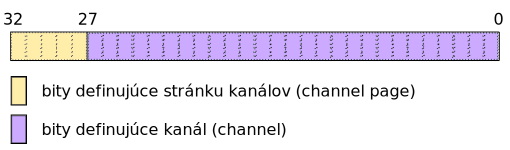
\includegraphics[width=120mm]{figures/channel_page}
\caption{32-bitový identifikátor kanálov a stránky kanálov}
\label{fig:channel_page}
\end{center}
\end{figure}
\begin{table}[htbp]
\begin{center}
\begin{tabular}{|c|c|c|c|c|}
  \hline
  \textbf{Stránka kanálu} & \textbf{Stránka kanálu} & \textbf{Číslo kanálu} & \textbf{Frekvenčné} & \\
  (dekadicky) & (binárne) & (dekadicky) & \textbf{pásmo} & \raisebox{1.5ex}{\textbf{Modulácia}} \\
  \hline
  \hline
  \multirow{3}{*}{0} & \multirow{3}{*}{0 0 0 0 0} & 0 & 868 MHz & BPSK \\
  \cline{3-5}
  & & 1--10 & 915 MHz & BPSK \\
  \cline{3-5}
  & & 11--26 &  2.4 GHz & O-QPSK \\ [0.5ex]
  \hline
  \multirow{3}{*}{1} & \multirow{3}{*}{0 0 0 0 1} & 0 & 868 MHz & ASK \\
  \cline{3-5}
  & & 1--10 & 915 MHz & ASK \\
  \cline{3-5}
  & & 11--26 & \multicolumn{2}{|c|}{Rezervované} \\ [0.5ex]
  \hline
  \multirow{3}{*}{2} & \multirow{3}{*}{0 0 0 1 0} & 0 & 868 MHz & O-QPSK \\
  \cline{3-5}
  & & 1--10 & 915 MHz & O-QPSK \\
  \cline{3-5}
  & & 11--26 & \multicolumn{2}{|c|}{Rezervované} \\ [0.5ex]
  \hline
  3--31 & 0 0 0 1 1 -- 1 1 1 1 1 & \multicolumn{3}{|c|}{Rezervované} \\ [0.5ex]
  \hline
\end{tabular}
\caption{Zoznam jednotlivých kombinácii kanálov, frekvenčných pásiem a použitých modulácii podľa nastavenia identifikátorov kanálov a stránky kanálov}
\label{tab:channel_page}
\end{center}
\end{table}
\subsection{Linková vrstva}
\indent\indent Linková vrstva IEEE 802.15.4b podľa~\cite{ieee06} je jednoduchá, ale flexibilná. Riadi a kontroluje prístup k zdieľanému médiu. K tomuto využíva nasledovné mechanizmy:
\begin{itemize}
\item Vysielanie beacon rámcov (periodicky, alebo neperiodicky v závislosti od aktuálnej konfigurácie siete)
\item Synchronizácia podľa beacon rámcov vysielaných svojimi susedmi
\item Podieľanie sa na procesoch asociácie a disasociácie v PAN sieti
\item V prípade požiadavku, podpora zabezpečenia
\item Prístup k médiu pomocou CSMA-CA algoritmu
\item Riadi a prideľuje GTS časové sloty 
\end{itemize}
\subsection{Beaconing a non-beaconing módy}
\indent\indent  Linková vrstva môže pracovať v dvoch základných režimoch - tzv. beaconing mód a~non-beaconing mód. Rozdiel medzi týmito módmi nie je v tom, či sú beacon rámce v~sieti posielané, ale v tom, či sú tieto rámce posielané pravidelne. V prípade, že je hodnota atribútu u koordinátora siete $macSuperframeOrder < macBeaconOrder$, to znamená, že sieť pracuje v beaconing móde a beacon rámce sú posielané pravidelne v~intervale vypočítanom podľa vzťahu 
$$ beaconPeriod = aBaseSuperframeDuration * 2^{macBeaconOrder}$$
kde výsledná hodnota intervalu je v symboloch. Podľa tabuľky~\ref{tab:frequencies} sa táto hodnota dá previesť na čas v sekundách. Hodnota konštanty aBaseSuperframeDuration je $960$ a~predstavuje dĺžku najkratšieho možného intervalu v symboloch oddeľujúceho začiatky dvoch beacon rámcov.\\
\indent Alternatívu predstavujú zhodné hodnoty atribútov \textit{macBeaconOrder} a \textit{macSuperframeOrder}. Vtedy sa jedná o non-beaconing mód a beacon rámce sa posielajú len ako odpoveď na explicitnú požiadavku o ich zaslanie.\\
\subsection{Superframe rámec}
\indent\indent Nami navrhovaný model uvažuje použitie beaconing módu, ktorý ponúka zaujímavejší mechanizmus komunikácie a využíva možnosti dané periodicitou v zasielaní riadiacich a kontrolných beacon rámcov. V tomto beaconing móde sa využíva komunikačná štruktúra, ktorá sa nazýva superframe rámec. Superframe rámec vymedzuje 4 periodicky sa opakujúce úseky (obr.~\ref{fig:superframe}) a pre každý z nich platia pravidlá pre posielanie a príjem dát. Superframe rámec vždy obsahuje 16 superframe slotov o dĺžke $aBaseSlotDuration * 2^{macSuperframeOrder}$ symbolov dynamicky distribuovaných do Contention Access periódy a Contention Free periódy. Slot, v ktorom je vysielaný beacon rámec je označovaný ako slot 0. Konštanta \textit{aBaseSlotDuration} má hodnotu $60$.\\
\begin{figure}[htbp]
\begin{center}
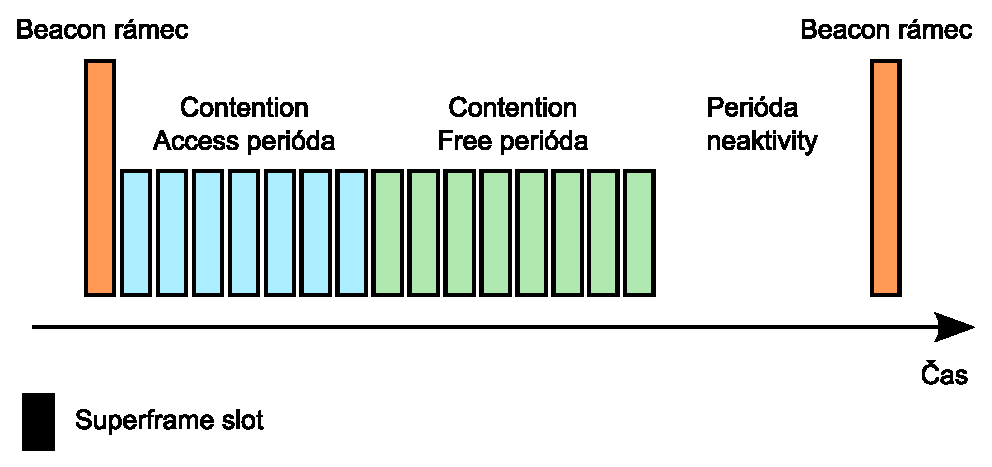
\includegraphics[width=140mm]{figures/superframe}
\caption{Štruktúra superframe rámca (obrázok nie je v mierke)}
\label{fig:superframe}
\end{center}
\end{figure}
\subsubsection{Beacon rámec}
\indent\indent Na úvod každého superframe rámca je FFD prvkom, ktorý je v sieti pripojený ako smerovač (router), posielaný beacon rámec. Obsahuje informačné polia, ktoré okrem iného obsahujú atribúty \textit{macBeaconOrder} a \textit{macSuperframeOrder} definujúce isté vlastnosti danej PAN siete. Z týchto polí vychádzajú hraničné časovače určujúce dĺžky jednotlivých úsekov superframe rámca. Okrem toho definuje aj koniec Contention Access periódy pomocou identifikátora \textit{FinalCAPSlot}.\\
\indent Beacon rámec je vysielaný prvkom bez použitia CSMA metódy, pretože všetky prvky v dosahu vysielača daného FFD prvku by sa mali synchronizovať na periodicitu týchto rámcov a nevysielať žiadne dáta na prenosové médium v čase, keď sa očakáva beacon rámec.\\
\paragraph{Contention Access perióda}
Počas tejto periódy prvky môžu pristupovať na médium pomocou metódy CSMA-CA. Tento moment slúži hlavne na vybavovanie žiadosti o asociáciu do siete, prípadne žiadosti o prenos užitočných dát smerom od FFD prvku. V takom prípade sú dáta, ktoré chce FFD poslať svojim susedom indikované v beacon rámci. FFD prvky majú väčšinou fronty na zasielanie týchto rámcov s užitočnými dátami pre koncové zariadenia. Ak si sused daného smerovača nevyžiada dáta po uplynutí nejakého konkrétneho počtu superframe rámcov od ich prvého indikovania v beacon rámci, smerovač ich z tejto fronty zahadzuje.\\
\indent Prvok, ktorému smerovač v beacon rámci neindikoval, že má pre neho vo svojich frontách zaradené dáta, a tento prvok ani nemá záujem žiadne dáta poslať smerom k~FFD zariadeniu môže vypnúť svoje vysielacie a prijímacie obvody a šetriť tak energiu.\\
\paragraph{Contention Free perióda}
Časový interval v ktorom sa prenášajú dáta pomocou mechanizmu GTS (Guaranteed Time Slot) sa nazýva Contention Free perióda. GTS mechanizmus alokuje určitý počet superframe slotov pre prenos dát, ktoré často majú periodický charakter. Beacon rámec posielaný smerovačom na úvod superframe rámca definuje aj počet alokovaných superframe slotov združených do GTS slotov a pre každý z týchto GTS slotov pomocou 16-bitovej, alebo 64-bitovej adresy určí druhú stranu komunikačného toku. Pomocou jednoduchej bitovej mapy je následne určený smer komunikácie (smerom od smerovača/smerom k smerovaču). GTS mechanizmus je v novom štandarde IEEE 802.15.4b-2006 vedený už len ako dobrovoľný spôsob prístupu k prenosu dát.\\

\section{ZigBee}
\indent\indent Medzi štandardy definujúce vyššie vrstvy komunikácie v LR-WPAN sieťach patrí napríklad ZigBee od združenia ZigBee Alliance~\cite{zigbee08}. Tento štandard definuje sieťovú a~aplikačnú vrstvu siete ZigBee a v prípade linkovej a sieťovej vrstvy sa spolieha na už vyššie popísaný štandard IEEE 802.15.4. Vzťah medzi ZigBee a IEEE 802.15.4 by sa dal prirovnať vzťahu medzi Wi-Fi a IEEE 802.11. Na obr.~\ref{fig:zigbee_ieee} je vyobrazený vzťah medzi vrstvami definovanými v ZigBee a IEEE štandardoch. Prvá z finálnych verzii ZigBee štandardu sa objavila koncom roku 2004, ale odvtedy bola ešte niekoľko krát upravovaná. My v tomto dokumente pracujeme s verziou z januára 2008~\cite{zigbee08}, momentálne najaktuálnejšou.\\
\begin{figure}[htbp]
\begin{center}
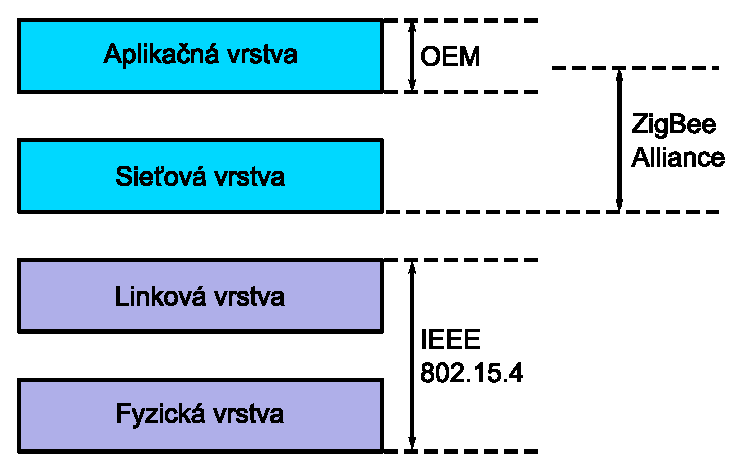
\includegraphics[width=140mm]{figures/zigbee_ieee}
\caption{Vzťah medzi ZigBee Alliance a IEEE 802.15.4}
\label{fig:zigbee_ieee}
\end{center}
\end{figure}
\indent Svojou charakteristikou sú siete ZigBee vhodné pre aplikácie nevyžadujúce vysoké nároky na datovú priepustnosť, uspokoja sa s bezdrôtovým spojením krátkeho dosahu, ale hlavne pre ktoré je kritická nízka energetická náročnosť. Tieto špecifiká posúvajú sie\-te ZigBee ako vhodného kandidáta pre bezdrôtové riadenie osvetlenia, termoreguláciu, bezpečnostné prvky v inteligentných domácnostiach, pre komunikáciu hlásičov požiaru v budovách, alebo aj v medicíne pre rýchle predávanie správ o stave pacienta do definovaného zberného bodu. V priemysle by zase táto technológia našla využitie napríklad v monitorovaní podmienok, v akých sa tovar nachádza v sklade (teplota, vlhkosť, vibrácie), alebo napríklad pri kontrole procesov v čističke odpadových vôd. Keďže sieť má vlastnosť samokonfigurácie, jej inštalácia aj vo väčších mierkach je otázkou zopár hodín.\\
\subsection{Architektúra ZigBee}
\indent\indent Architektúra siete ZigBee sa skladá zo štyroch základných vrstiev, ako zobrazuje aj obr.~\ref{fig:zigbee_ieee}. Tieto vrstvy medzi sebou komunikujú predávaním správ cez tzv. body prístupu služby (SAP - Service Access Point). SAP je v princípe miesto, v ktorom jedna v vrstiev môže požadovať služby druhej vrstvy. štruktúra architektúry spolu s vyznačenými SAP bodmi je vyobrazená na obrázku~\ref{fig:architecture_zigbee}. Na ňom môžme rozlišovať dva typy SAP bodov medzi jednotlivými vrstvami. Jeden typ predstavujú body, cez ktoré sú spracovávané užitočné dáta aplikácii (napr. MCPS-SAP, alebo PD-SAP) a druhý typ SAP bodov sa zaoberá manažmentom siete, ako napr. konfigurácia beacon rámcov, prípadne nastavovanie, alebo čítanie hodnôt atribútov (napr. MLME-SAP, PLME-SAP body).\\
\begin{figure}[htbp]
\begin{center}
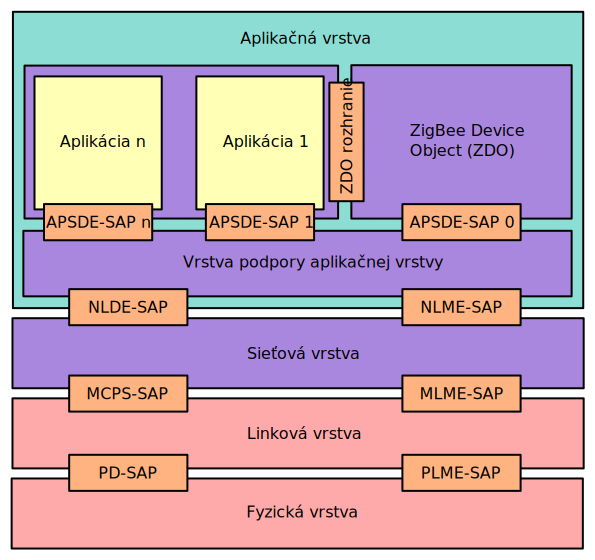
\includegraphics[width=140mm]{figures/architecture_zigbee}
\caption{Znázornenie vrstvovej architektúry siete ZigBee}
\label{fig:architecture_zigbee}
\end{center}
\end{figure}
\subsection{Sieťová vrstva}
\indent\indent Požiadavky na sieťovú vrstvu sú zabezpečovanie správneho fungovania linkovej vrstvy a poskytovania vhodných služieb vyššie postavenej aplikačnej vrstve. Podľa konceptu, sieťová vrstva obsahuje dve entity, ktorých služby sú využívané aplikačnou vrstvou. Tie\-to entity sú datová (NLDE - NWK Layer Data Entity) a manažement entita (NLME - NWK Layer Management Entity). Ku každej sa pristupuje cez príslušný bod SAP - NLDE-SAP, alebo NLME-SAP. Zmysel rozdelenia sieťovej vrstvy na tieto dve časti je v~tom, že NLME využíva NLDE pre vykonávanie potrebných úloh, ktoré majú charakter riadenia a kontroly na danej úrovni a takisto zabezpečuje prístup k sieťovej informačnej databázy (NIB - Network Information Base).\\
\subsection{Aplikačná vrstva}
\indent\indent Ako je ukázané na obrázku~\ref{fig:architecture_zigbee}, aplikačná vrstva sa skladá zo ZigBee Device Object objektu, z aplikačných objektov (definovaných výrobcom zariadenia, alebo aplikácie) a~z~podpornej vrstvy APS.\\
\subsubsection{Podporná vrstva aplikačnej vrstve}
\indent\indent Uvedená vrstva je v špecifikácii označovaná ako APS (Application Support Sub\-layer). Úlohy, ktoré jej prináležia si delia dve entity: datová (APSDE) a manažment (APSME). Datová ma na starosť sprístupnenie služieb pre aplikačné vrstvy v danej sieti a management entita zabezpečuje cez príslušný SAP bod funkcie bezpečnosti prenosu, prípadne prístup k informačnej báze danej podvrstvy. S podobným rozdelením sa budeme stretávať aj pri ostatných vrstvách protokolu.\\
\subsubsection{Objekty typu ZigBee Device Objects}
\indent\indent ZigBee Device Objects objekty (ZDO) hrajú dôležitú úlohu v protokole ZigBee. Pri štarte siete inicializujú sieťovú vrstvu a vrstvu APS. Na základe požiadavkov aplikácii dávajú impulz k procesom, ktoré realizujú vytváranie PAN, asociáciu do už existujúcej siete PAN, prípadne majú na starosť správu sieťovej vrstvy. Ako už bolo spomenuté v~\cite{halas03} ZDO môžme nazvať komunikačným bodom aplikačnej vrstvy. ZDO poskytuje funkcie pre všetky aplikácie bežiace na ZigBee zariadení vrátane skenovania siete (device and service discovery), vytvorenia spojení medzi objektami v sieti (binding) a správy šifrovacích kľúčov (security management). Vo výslednej simulácii je jediná z jej úloh inicializácia daného zariadenia spolu s nastavením základných parametrov pre spojenie. Na aplikačnej vrstve sú uvažované tzv. endpoints. Zariadenie môže mať nadefinovaných max. 240 endpoints a každému z nich zodpovedá jeden aplikačný profil. Pre ilustráciu môžme uviesť, že cez jeden endpoint je realizovaná komunikácia s cieľom zapnúť svetlo a cez iný endpoint môže aplikácia informovať iný ZigBee prvok o teplote prostredia zmeranej teplotným čidlom.\\
\subsection{Väzba na IEEE 802.15.4}
\indent\indent V špecifikácii k IEEE 802.15.4 sú uvedené aj doplnkové podvrstvy k základnéj vrstvovej štruktúre. Na mysli máme podvrstvy označované ako SSCS (Sublayer-Specific Convergence Layer) a LLC (Logical Link Control) vrstvy. Ich polohu znázorňuje obrázok~\ref{fig:architecture_sublayers}. Konvergenčná SSCS vrstva slúži k predávaniu informácii medzi sieťovou a~linkovou vrstvou. Následne má schopnosť informovať nadradené vrstvy o tom, v akom stave sa nachádza posielanie dát ostatným členom siete. Funkciou podvrstvy IEEE 802.2 LLC  je kontrola a zaistenie integrity dátových prenosov. LLC vrstva poskytuje cez body prístupu (SAP) služby linkovej vrstvy pre sieťovú vrstvu.\\
\begin{figure}[htbp]
\begin{center}
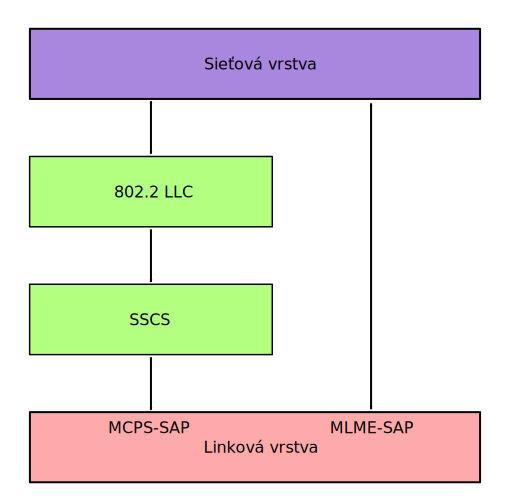
\includegraphics[width=120mm]{figures/architecture_sublayers}
\caption{Použitie doplňujúcich vrstiev v komunikácii medzi linkovou a sieťovou vrstvou}
\label{fig:architecture_sublayers}
\end{center}
\end{figure}

%*****************************************************************************
\chapter{Popis problému, specifikace cíle}

\begin{itemize}
\item Popis řešeného problému, vymezení cílů DP/BP a požadavků na implementovaný systém.
\item Popis struktury DP/BP ve vztahu k vytyčeným cílům.
\item Rešeršní zpracování existujících implementací, pokud jsou známy.
\end{itemize}

%*****************************************************************************
\chapter{Analýza a návrh řešení}
Analýza a návrh implementace (včetně diskuse různých alternativ a volby implementačního prostředí).


%*****************************************************************************
\chapter{Realizace}
Popis implementace / realizace se zaměřením na nestandardní části řešení.


%*****************************************************************************
\chapter{Testování}

\begin{itemize}
 \item Způsob, průběh a výsledky testování.
 \item Srovnání s existujícími řešeními, pokud jsou známy.
\end{itemize} 


%*****************************************************************************
\chapter{Závěr}

\begin{itemize}
\item Zhodnocení splnění cílů DP/BP a  vlastního přínosu práce (při formulaci je třeba vzít v potaz zadání práce).
\item Diskuse dalšího možného pokračování práce.
\end{itemize} 

%*****************************************************************************
% Seznam literatury je v samostatnem souboru reference.bib. Ten
% upravte dle vlastnich potreb, potom zpracujte (a do textu
% zapracujte) pomoci prikazu bibtex a nasledne pdflatex (nebo
% latex). Druhy z nich alespon 2x, aby se poresily odkazy.

\bibliographystyle{abbrv}
%bibliographystyle{plain}
%\bibliographystyle{psc}
{
%JZ: 11.12.2008 (Nekdo chce mit v techto ukazkovych odkazech take odkaz 
%JZ: na CSTeX, tak at to k necemu vypada...)
\def\CS{$\cal C\kern-0.1667em\lower.5ex\hbox{$\cal S$}\kern-0.075em $}
\bibliography{reference}
}

% M. Dušek radi:
%\bibliographystyle{alpha}
% kdy citace ma tvar [AutorRok] (napriklad [Cook97]). Sice to asi neni  podle ceske normy (BTW BibTeX stejne neodpovida ceske norme), ale je to nejprehlednejsi.


%*****************************************************************************
%*****************************************************************************
\appendix

\chapter{Testování zaplnění stránky a odsazení odstavců}
\textbf{\large Tato příloha samozřejmě nebude součástí vaší práce. Slouží pouze jako příklad formátování textu.}

% 11.12.2008 JZ rucne: osetreni uderfull vboxu.
\section*{}
Určitě existuje nějaká pěkná latinská věta, která se k tomuhle testování používá, ale co mají dělat ti, kteří se nikdy latinsky neučili? Určitě existuje nějaká pěkná latinská věta, která se k tomuhle testování používá, ale co mají dělat ti, kteří se nikdy latinsky neučili? Určitě existuje nějaká pěkná latinská věta, která se k tomuhle testování používá, ale co mají dělat ti, kteří se nikdy latinsky neučili?

Určitě existuje nějaká pěkná latinská věta, která se k tomuhle testování používá, ale co mají dělat ti, kteří se nikdy latinsky neučili? Určitě existuje nějaká pěkná latinská věta, která se k tomuhle testování používá, ale co mají dělat ti, kteří se nikdy latinsky neučili? Určitě existuje nějaká pěkná latinská věta, která se k tomuhle testování používá, ale co mají dělat ti, kteří se nikdy latinsky neučili?

Určitě existuje nějaká pěkná latinská věta, která se k tomuhle testování používá, ale co mají dělat ti, kteří se nikdy latinsky neučili? Určitě existuje nějaká pěkná latinská věta, která se k tomuhle testování používá, ale co mají dělat ti, kteří se nikdy latinsky neučili? Určitě existuje nějaká pěkná latinská věta, která se k tomuhle testování používá, ale co mají dělat ti, kteří se nikdy latinsky neučili?

Určitě existuje nějaká pěkná latinská věta, která se k tomuhle testování používá, ale co mají dělat ti, kteří se nikdy latinsky neučili? Určitě existuje nějaká pěkná latinská věta, která se k tomuhle testování používá, ale co mají dělat ti, kteří se nikdy latinsky neučili? Určitě existuje nějaká pěkná latinská věta, která se k tomuhle testování používá, ale co mají dělat ti, kteří se nikdy latinsky neučili? Určitě existuje nějaká pěkná latinská věta, která se k tomuhle testování používá, ale co mají dělat ti, kteří se nikdy latinsky neučili? Určitě existuje nějaká pěkná latinská věta, která se k tomuhle testování používá, ale co mají dělat ti, kteří se nikdy latinsky neučili? Určitě existuje nějaká pěkná latinská věta, která se k tomuhle testování používá, ale co mají dělat ti, kteří se nikdy latinsky neučili?

Určitě existuje nějaká pěkná latinská věta, která se k tomuhle testování používá, ale co mají dělat ti, kteří se nikdy latinsky neučili? Určitě existuje nějaká pěkná latinská věta, která se k tomuhle testování používá, ale co mají dělat ti, kteří se nikdy latinsky neučili?

Určitě existuje nějaká pěkná latinská věta, která se k tomuhle testování používá, ale co mají dělat ti, kteří se nikdy latinsky neučili? Určitě existuje nějaká pěkná latinská věta, která se k tomuhle testování používá, ale co mají dělat ti, kteří se nikdy latinsky neučili? Určitě existuje nějaká pěkná latinská věta, která se k tomuhle testování používá, ale co mají dělat ti, kteří se nikdy latinsky neučili? Určitě existuje nějaká pěkná latinská věta, která se k tomuhle testování používá, ale co mají dělat ti, kteří se nikdy latinsky neučili? Určitě existuje nějaká pěkná latinská věta, která se k tomuhle testování používá, ale co mají dělat ti, kteří se nikdy latinsky neučili?

%*****************************************************************************
\chapter{Pokyny a návody k formátování textu práce}
\textbf{\large Tato příloha samozřejmě nebude součástí vaší práce. Slouží pouze jako příklad formátování textu.}

Používat se dají všechny příkazy systému \LaTeX. Existuje velké množství volně přístupné dokumentace, tutoriálů, příruček a dalších materiálů v elektronické podobě. Výchozím bodem, kromě Googlu, může být stránka CSTUG (Czech Tech Users Group) \cite{CSTUG}. Tam najdete odkazy na další materiály.  Vetšinou dostačující a přehledně organizovanou elektronikou dokumentaci najdete například na \cite{latexdocweb} nebo \cite{latexwiki}.

Existují i různé nadstavby nad systémy \TeX{} a \LaTeX, které výrazně usnadní psaní textu zejména začátečníkům. Velmi rozšířený v Linuxovém prostředí je systém Kile.


\section{Vkládání obrázků}
Obrázky se umísťují do plovoucího prostředí \verb|figure|. Každý obrázek by měl obsahovat \textbf{název} (\verb|\caption|) a \textbf{návěští} (\verb|\label|). Použití příkazu pro vložení obrázku \\\verb|\includegraphics| je podmíněno aktivací (načtením) balíku graphicx příkazem\\ \verb|\usepackage{graphicx}|.

Budete-li zdrojový text zpracovávat pomocí programu \verb|pdflatex|, očekávají se obrázky s příponou \verb|*.pdf|\footnote{pdflatex umí také formáty PNG a JPG.}, použijete-li k formátování \verb|latex|, očekávají se obrázky s příponou \verb|*.eps|.\footnote{Vzájemnou konverzi mezi snad všemi typy obrazku včetně změn vekostí a dalších vymožeností vám může zajistit balík ImageMagic  (http://www.imagemagick.org/script/index.php). Je dostupný pod Linuxem, Mac OS i MS Windows. Důležité jsou zejména příkazy convert a identify.}

\begin{figure}[ht]
\begin{center}

\includegraphics[width=5cm]{figures/LogoCVUT}
\caption{Popiska obrázku}
\label{fig:logo}
\end{center}
\end{figure}

Příklad vložení obrázku:
\begin{verbatim}
\begin{figure}[h]
\begin{center}

\includegraphics[width=5cm]{figures/LogoCVUT}
\caption{Popiska obrazku}
\label{fig:logo}
\end{center}
\end{figure}
\end{verbatim}

\section{Kreslení obrázků}
Zřejmě každý z vás má nějaký oblíbený nástroj pro tvorbu obrázků. Jde jen o to, abyste dokázali obrázek uložit v požadovaném formátu nebo jej do něj konvertovat (viz předchozí kapitola). Je zřejmě vhodné kreslit obrázky vektorově. Celkem oblíbený, na ovládání celkem jednoduchý a přitom dostatečně mocný je například program Inkscape.

Zde stojí za to upozornit na kreslící programe Ipe \cite{ipe}, který dokáže do obrázku vkládat komentáře přímo v latexovském formátu (vzroce, stejné fonty atd.). Podobné věci umí na Linuxové platformě nástroj Xfig. 

Za pozornost ještě stojí schopnost editoru Ipe importovat obrázek (jpg nebo bitmap) a krelit do něj latexovské popisky a komentáře. Výsledek pak umí exportovat přímo do pdf.

\section{Tabulky}
Existuje více způsobů, jak sázet tabulky. Například je možno použít prostředí \verb|table|, které je velmi podobné prostředí \verb|figure|. 

\begin{table}
\begin{center}
\begin{tabular}{|c|l|l|}
\hline
\textbf{DTD} & \textbf{construction} & \textbf{elimination} \\
\hline
$\mid$ & \verb+in1|A|B a:sum A B+ & \verb+case([_:A]a)([_:B]a)ab:A+\\
&\verb+in1|A|B b:sum A B+ & \verb+case([_:A]b)([_:B]b)ba:B+\\
\hline
$+$&\verb+do_reg:A -> reg A+&\verb+undo_reg:reg A -> A+\\
\hline
$*,?$& the same like $\mid$ and $+$ & the same like $\mid$ and $+$\\
& with \verb+emtpy_el:empty+ & with \verb+emtpy_el:empty+\\
\hline
R(a,b) & \verb+make_R:A->B->R+ & \verb+a: R -> A+\\
 & & \verb+b: R -> B+\\
\hline
\end{tabular}
\end{center}
\caption{Ukázka tabulky}
\label{tab:tab1}
\end{table}

Zdrojový text tabulky \ref{tab:tab1} vypadá takto:
\begin{verbatim}
\begin{table}
\begin{center}
\begin{tabular}{|c|l|l|}
\hline
\textbf{DTD} & \textbf{construction} & \textbf{elimination} \\
\hline
$\mid$ & \verb+in1|A|B a:sum A B+ & \verb+case([_:A]a)([_:B]a)ab:A+\\
&\verb+in1|A|B b:sum A B+ & \verb+case([_:A]b)([_:B]b)ba:B+\\
\hline
$+$&\verb+do_reg:A -> reg A+&\verb+undo_reg:reg A -> A+\\
\hline
$*,?$& the same like $\mid$ and $+$ & the same like $\mid$ and $+$\\
& with \verb+emtpy_el:empty+ & with \verb+emtpy_el:empty+\\
\hline
R(a,b) & \verb+make_R:A->B->R+ & \verb+a: R -> A+\\
 & & \verb+b: R -> B+\\
\hline
\end{tabular}
\end{center}
\caption{Ukázka tabulky}
\label{tab:tab1}
\end{table}
\begin{table}
\end{verbatim}

\section{Odkazy v textu}
\subsection{Odkazy na literaturu}
Jsou realizovány příkazem \verb|\cite{odkaz}|. 

Seznam literatury je dobré zapsat do samostatného souboru a ten pak zpracovat programem bibtex (viz soubor \verb|reference.bib|). Zdrojový soubor pro \verb|bibtex| vypadá například takto:
\begin{verbatim}
@Article{Chen01,
  author  = {Yong-Sheng Chen and Yi-Ping Hung and Chiou-Shann Fuh},
  title   = {Fast Block Matching Algorithm Based on the Winner-Update 
             Strategy},
  journal = {IEEE Transactions On Image Processing},
  pages   = {1212--1222},
  volume  =   10,
  number  =    8,
  year    = 2001,
}

@Misc{latexdocweb,
  author =       {},
  title =        {{\LaTeX} --- online manuál},
  note =         {\verb|http://www.cstug.cz/latex/lm/frames.html|},
  year =         {},
}
....
\end{verbatim}

%11.12.2008 JZ rucne
\textbf{Pozor:} \ Budete-li \ používat \ české \ prostředí (\verb|\usepackage[czech]{babel}|), potom \verb|bibtex| automaticky vysází s velké pouze počáteční písmeno z názvu zdroje, ostatní písmena zůstanou malá bez ohledu na to, jak je napíšete. Pokud to chcete jinak (viz \verb|title = {{LaTeX - online manuál}},| v~předchozím příkladu), je nutné text uzavřít do dvojitých složených závorek.

Odkazy na literaturu ve zdrojovém textu se pak zapisují:
\begin{verbatim}
Podívejte se na \cite{Chen01}, 
další detaily najdete na \cite{latexdocweb}
\end{verbatim}

Vazbu mezi soubory \verb|*.tex| a \verb|*.bib| zajistíte příkazem  \verb|\bibliography{}| v souboru \verb|*.tex|.  V našem případě tedy zdrojový dokument \verb|thesis.tex| obsahuje příkaz\\  \verb|\bibliography{reference}|.

Zpracování zdrojového textu s odkazy se provede postupným voláním programů\\
\verb|pdflatex <soubor>| (případně \verb|latex <soubor>|), \verb|bibtex <soubor>| a opět\\ \verb|pdflatex <soubor>|.\footnote{První volání pdflatex vytvoří soubor s koncovkou *.aux, který je vstupem pro program bibtex, pak je potřeba znovu zavolat program pdflatex (latex), který tentokrát zpracuje soubory s příponami .aux a .tex. Informaci o případných nevyřešených odkazech (cross-reference) vidíte přímo při zpracovávání zdrojového souboru příkazem pdflatex. Program pdflatex (latex) lze volat vícekrát, pokud stále vidíte nevyřešené závislosti.}


Níže uvedený příklad je převzat z dříve existujících pokynů studentům, kteří dělají svou  diplomovou nebo bakalářskou práci v Grafické skupině. \footnote{Několikrát jsem byl upozorněn, že web s těmito pokyny byl zrušen, proto jej zde přímo necituji. Nicméně příklad sám o sobě dokumentuje obecně přijímaný koncesus ohledně citací v bakalářských a diplomových pacích na KP.} Zde se praví:
\begin{small}
\begin{verbatim}
...
j) Seznam literatury a dalších použitých pramenů, odkazy na WWW stránky, ...
 Pozor na to, že na veškeré uvedené prameny se musíte v textu práce 
 odkazovat -- [1]. 
Pramen, na který neodkazujete, vypadá, že jste ho vlastně nepotřebovali 
a je uveden jen do počtu. Příklad citace knihy [1], článku v časopise [2], 
stati ve sborníku [3] a html odkazu [4]: 
[1] J. Žára, B. Beneš;, and P. Felkel. 
     Moderní počítačová grafika. Computer Press s.r.o, Brno, 1 edition, 1998. 
     (in Czech). 
[2] P. Slavík. Grammars and Rewriting Systems as Models for Graphical User 
     Interfaces. Cognitive Systems, 4(4--3):381--399, 1997. 
[3] M. Haindl, Š. Kment, and P. Slavík. Virtual Information Systems. 
     In WSCG'2000 -- Short communication papers, pages 22--27, Pilsen, 2000. 
     University of West Bohemia. 
[4] Knihovna grafické skupiny katedry počítačů: 
     http://www.cgg.cvut.cz/Bib/library/ 
\end{verbatim}
\end{small}
\ldots{} abychom výše citované odkazy skutečně našli v (automaticky generovaném) seznamu literatury tohoto textu, musíme je nyní alespoň jednou citovat: Kniha \cite{kniha}, článek v~časopisu \cite{clanek}, příspěvek na konferenci \cite{sbornik}, www odkaz \cite{www}.

\subsection{Odkazy na obrázky, tabulky a kapitoly}
\begin{itemize}
\item Označení místa v textu, na které chcete později čtenáře práce odkázat, se provede příkazem \verb|\label{navesti}|. Lze použít v prostředích \verb|figure| a  \verb|table|, ale též za názvem kapitoly nebo podkapitoly.
\item Na návěští se odkážeme příkazem \verb|\ref{navesti}| nebo \verb|\pageref{navesti}|.
\end{itemize}

\section{Rovnice, centrovaná, číslovaná matematika}
Jednoduchý matematický výraz zapsaný přímo do textu se vysází pomocí prostředí \verb|math|, resp. zkrácený zápis pomocí uzavření textu rovnice mezi znaky \verb|$|.

Kód \verb|$ S = \pi * r^2 $| bude vysázen takto: $ S = \pi * r^2 $.

Pokud chcete nečíslované rovnice, ale umístěné centrovaně na samostatné řádky, pak lze použít prostředí \verb|displaymath|, resp. zkrácený zápis pomocí uzavření textu rovnice mezi znaky \verb|$$|. Zdrojový kód: 
\begin{verb}
|$$ S = \pi * r^2 $$|
\end{verb}
bude pak vysázen takto:
$$ S = \pi * r^2 $$

Chcete-li mít rovnice číslované, je třeba použít prostředí \verb|eqation|. Kód:
\begin{verbatim}
\begin{equation}
  S = \pi * r^2
\end{equation}

\begin{equation}
  V = \pi * r^3
\end{equation}
\end{verbatim}
je potom vysázen takto:
\begin{equation}
  S = \pi * r^2
\end{equation}

\begin{equation}
  V = \pi * r^3
\end{equation}

\section{Kódy programu}
Chceme-li vysázet například část zdrojového kódu programu (bez formátování), hodí se prostředí \verb|verbatim|: 
\begin{verbatim}
         (* nickname2 *)
Lego> Refine in1
             (do_reg (nickname1 h));
Refine by  in1 (do_reg (nickname1 h))
   ?4 : pcdata
   ?5 : pcdata
          (* surname2 *)
Lego> Refine surname1 h;
Refine by  surname1 h
   ?5 : pcdata
          (* email2 *)
Lego> Refine undo_reg (email1 h);
Refine by  undo_reg (email1 h)
*** QED ***
\end{verbatim}

\section{Další poznámky}
\subsection{České uvozovky}
V souboru \verb|k336_thesis_macros.tex| je příkaz \verb|\uv{}| pro sázení českých uvozovek. \uv{Text uvavřený do českých uvozovek.}

\subsection{Začátky kapitol na liché stránky}
Ve výsledném textu je dobré, když každá kapitola začíná na liché stránce. Tedy pouzijte:
\begin{verbatim}
  \cleardoublepage\include{1_uvod}
  \cleardoublepage\include{2_teorie}
   atd.\ldots{}
\end{verbatim}

%*****************************************************************************
\chapter{Zoznam použitých skratiek}

\begin{description}
\item[APP] Application
\item[CSMA-CA] Carrier Sense Multiple Access - Collision Avoidance
\item[FFD] Full Functionality Device
\item[GTS] Guaranteed Time Slot
\item[IEEE] Institute of Electrical and Electronics Engineers
\item[ISM] Industrial Scientific and Medical
\item[LR-WPAN] Low-Rate Wireless Personal Area Network
\item[MAC] Medium Access Control
\item[MHz] Megahertz
\item[NET] Network
\item[PAN] Personal Area network
\item[PHY] Physical
\item[RFD] Reduced Functionality Device
\item[UWB] Ultra-Wideband
\item[WPAN] Wireless Personal Area Network
\end{description}
\vdots

%*****************************************************************************
\chapter{UML diagramy}
\textbf{\large Tato příloha není povinná a zřejmě se neobjeví v každé práci. Máte-li ale větší množství podobných diagramů popisujících systém, není nutné všechny umísťovat do hlavního textu, zvláště pokud by to snižovalo jeho čitelnost.}

%*****************************************************************************
\chapter{Instalační a uživatelská příručka}
\textbf{\large Tato příloha velmi žádoucí zejména u softwarových implementačních prací.}

%*****************************************************************************
\chapter{Obsah přiloženého CD}
\textbf{\large Tato příloha je povinná pro každou práci. Každá práce musí totiž obsahovat přiložené CD. Viz dále.}

Může vypadat například takto. Váš seznam samozřejmě bude odpovídat typu vaší práce. (viz \cite{infodp}):

\begin{figure}[h]
\begin{center}
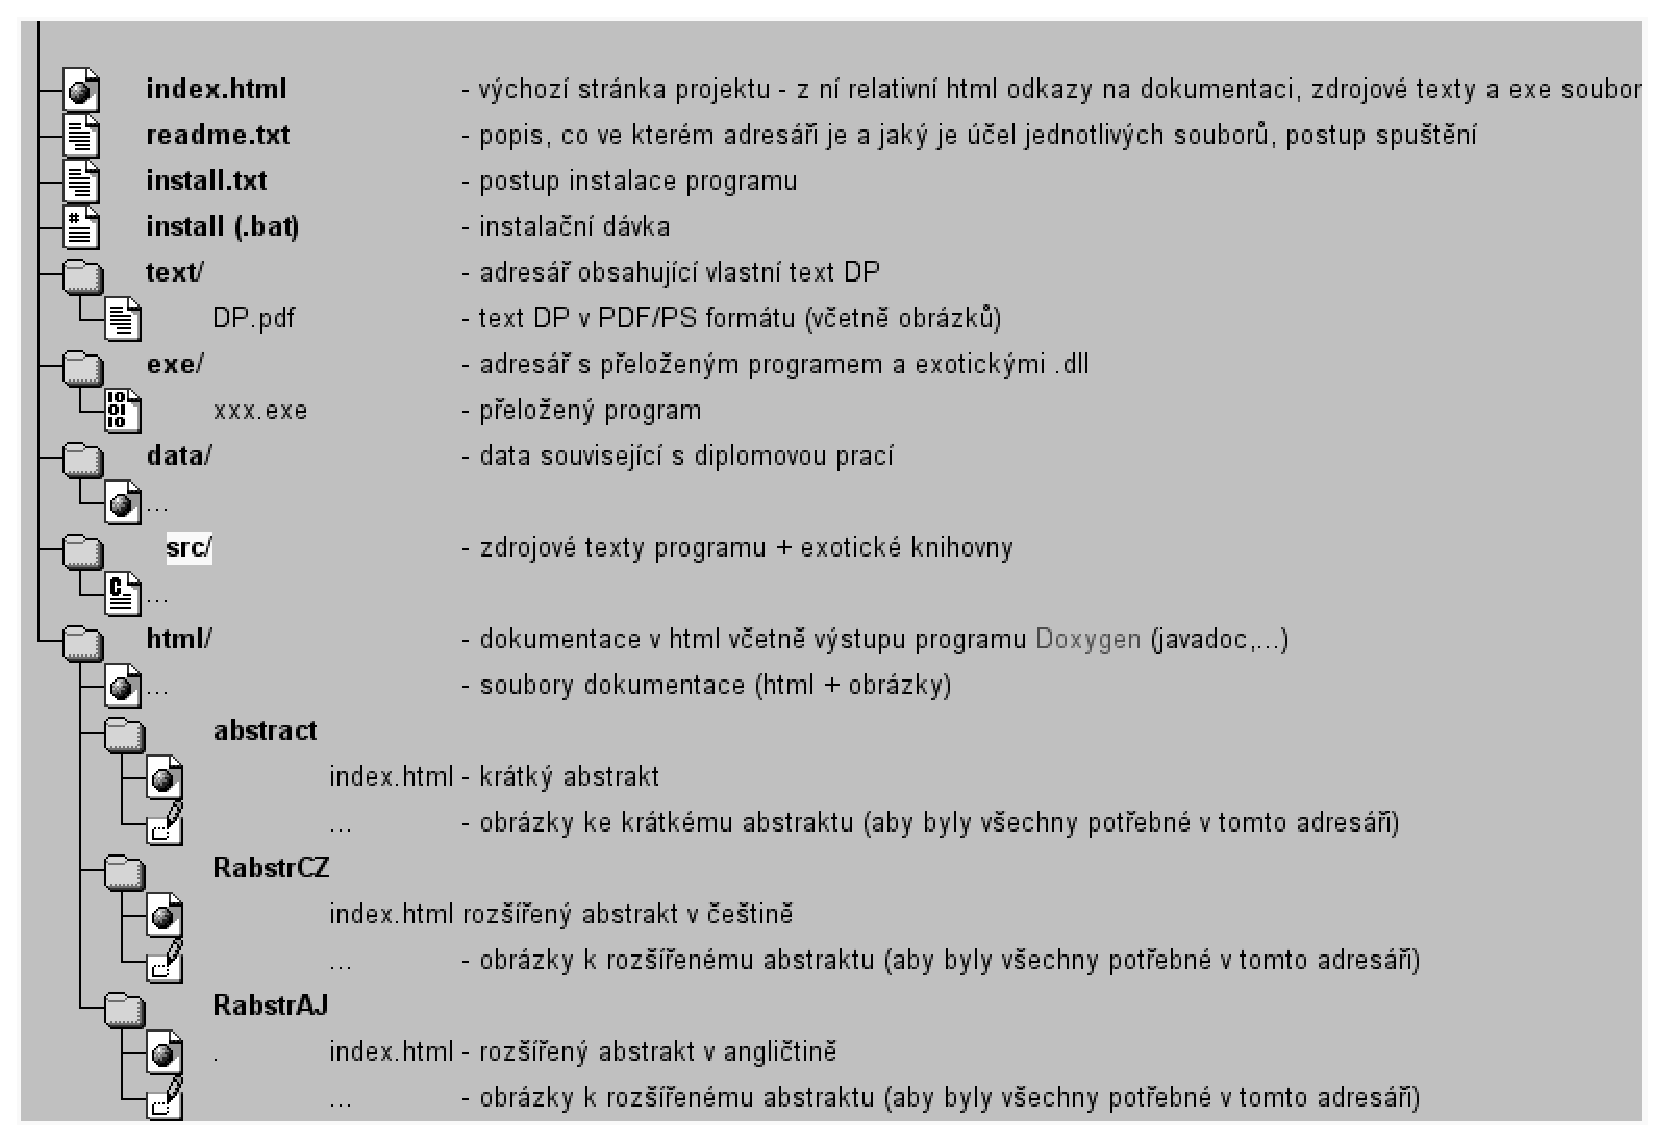
\includegraphics[width=14cm]{figures/seznamcd}
\caption{Seznam přiloženého CD --- příklad}
\label{fig:seznamcd}
\end{center}
\end{figure}

Na GNU/Linuxu si strukturu přiloženého CD můžete snadno vyrobit příkazem:\\ 
\verb|$ tree . >tree.txt|\\
Ve vzniklém souboru pak stačí pouze doplnit komentáře.

Z \textbf{README.TXT} (případne index.html apod.)  musí být rovněž zřejmé, jak programy instalovat, spouštět a jaké požadavky mají tyto programy na hardware.

Adresář \textbf{text}  musí obsahovat soubor s vlastním textem práce v PDF nebo PS formátu, který bude později použit pro prezentaci diplomové práce na WWW.

\end{document}
